%% Creator: Inkscape 0.91, www.inkscape.org
%% PDF/EPS/PS + LaTeX output extension by Johan Engelen, 2010
%% Accompanies image file 'Vzorkovani_prekryvani.pdf' (pdf, eps, ps)
%%
%% To include the image in your LaTeX document, write
%%   \input{<filename>.pdf_tex}
%%  instead of
%%   \includegraphics{<filename>.pdf}
%% To scale the image, write
%%   \def\svgwidth{<desired width>}
%%   \input{<filename>.pdf_tex}
%%  instead of
%%   \includegraphics[width=<desired width>]{<filename>.pdf}
%%
%% Images with a different path to the parent latex file can
%% be accessed with the `import' package (which may need to be
%% installed) using
%%   \usepackage{import}
%% in the preamble, and then including the image with
%%   \import{<path to file>}{<filename>.pdf_tex}
%% Alternatively, one can specify
%%   \graphicspath{{<path to file>/}}
%%
%% For more information, please see info/svg-inkscape on CTAN:
%%   http://tug.ctan.org/tex-archive/info/svg-inkscape
%%
\begingroup%
  \makeatletter%
  \providecommand\color[2][]{%
    \errmessage{(Inkscape) Color is used for the text in Inkscape, but the package 'color.sty' is not loaded}%
    \renewcommand\color[2][]{}%
  }%
  \providecommand\transparent[1]{%
    \errmessage{(Inkscape) Transparency is used (non-zero) for the text in Inkscape, but the package 'transparent.sty' is not loaded}%
    \renewcommand\transparent[1]{}%
  }%
  \providecommand\rotatebox[2]{#2}%
  \ifx\svgwidth\undefined%
    \setlength{\unitlength}{256bp}%
    \ifx\svgscale\undefined%
      \relax%
    \else%
      \setlength{\unitlength}{\unitlength * \real{\svgscale}}%
    \fi%
  \else%
    \setlength{\unitlength}{\svgwidth}%
  \fi%
  \global\let\svgwidth\undefined%
  \global\let\svgscale\undefined%
  \makeatother%
  \begin{picture}(1,0.4375)%
    \put(0.81750077,0.08750001){\color[rgb]{0,0,0}\makebox(0,0)[lb]{\smash{}}}%
    \put(0.81562436,0.0251556){\color[rgb]{0,0,0}\makebox(0,0)[lb]{\smash{}}}%
    \put(1.10953212,1.08921874){\color[rgb]{0,0,0}\makebox(0,0)[lb]{\smash{}}}%
    \put(0.51187664,1.08921874){\color[rgb]{0,0,0}\makebox(0,0)[lb]{\smash{}}}%
    \put(1.35562718,1.08921874){\color[rgb]{0,0,0}\makebox(0,0)[lb]{\smash{}}}%
    \put(0.11875,0.25){\color[rgb]{0,0,0}\makebox(0,0)[lb]{\smash{}}}%
    \put(0,0){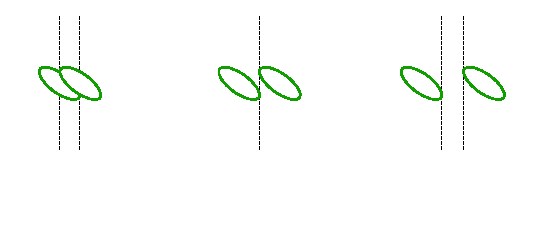
\includegraphics[width=\unitlength,page=1]{Vzorkovani_prekryvani.pdf}}%
    \put(0.12727737,0.42111206){\color[rgb]{0,0,0}\makebox(0,0)[b]{\smash{\textbf A)}}}%
    \put(0.48582077,0.42111206){\color[rgb]{0,0,0}\makebox(0,0)[b]{\smash{\textbf B)}}}%
    \put(0.84499741,0.42111206){\color[rgb]{0,0,0}\makebox(0,0)[b]{\smash{\textbf C)}}}%
    \put(0.05878548,-0.06382422){\color[rgb]{0,0,0}\makebox(0,0)[b]{\smash{}}}%
    \put(0.125,0.09375){\color[rgb]{0,0,0}\makebox(0,0)[b]{\smash{$\Delta x>\frac{1}{2W_{u}}$}}}%
    \put(0.125,0.03125){\color[rgb]{0,0,0}\makebox(0,0)[b]{\smash{$\Delta x>\frac{1}{2W_{u}}$}}}%
    \put(0.48486632,0.09375){\color[rgb]{0,0,0}\makebox(0,0)[b]{\smash{$\Delta x=\frac{1}{2W_{u}}$}}}%
    \put(0.48486632,0.03125){\color[rgb]{0,0,0}\makebox(0,0)[b]{\smash{$\Delta x=\frac{1}{2W_{u}}$}}}%
    \put(0.84424132,0.09375){\color[rgb]{0,0,0}\makebox(0,0)[b]{\smash{$\Delta x<\frac{1}{2W_{u}}$}}}%
    \put(0.84424132,0.03125){\color[rgb]{0,0,0}\makebox(0,0)[b]{\smash{$\Delta x<\frac{1}{2W_{u}}$}}}%
  \end{picture}%
\endgroup%
